Sea la función $G$:

\begin{equation}
    G(s) = \frac{s^2 + s + 1}{s^3 + 0.5s^2 + 3}
\end{equation}


La razón por la que el sistema es inestable para $H = 1$ es porque tiene polos con parte real positiva, por lo tanto el sistema no es estable. En cambio, cuando $H = 6$, el sistema se hace estable ya que los polos se mueve del semiplano derecho del plano complejo al izquierdo, representando estabilidad.

Ahora, sea el mismo sistema pero el compensador $H$ cambia de valor según el bucle \texttt{for c = 3:0.5:9}. La Figura \ref{fig:1} muestra el lugar de raíces (discreto) para el sistema definido por $G$ cuando $H$ cambia de valor:

\begin{figure}[ht!]
    \centering
    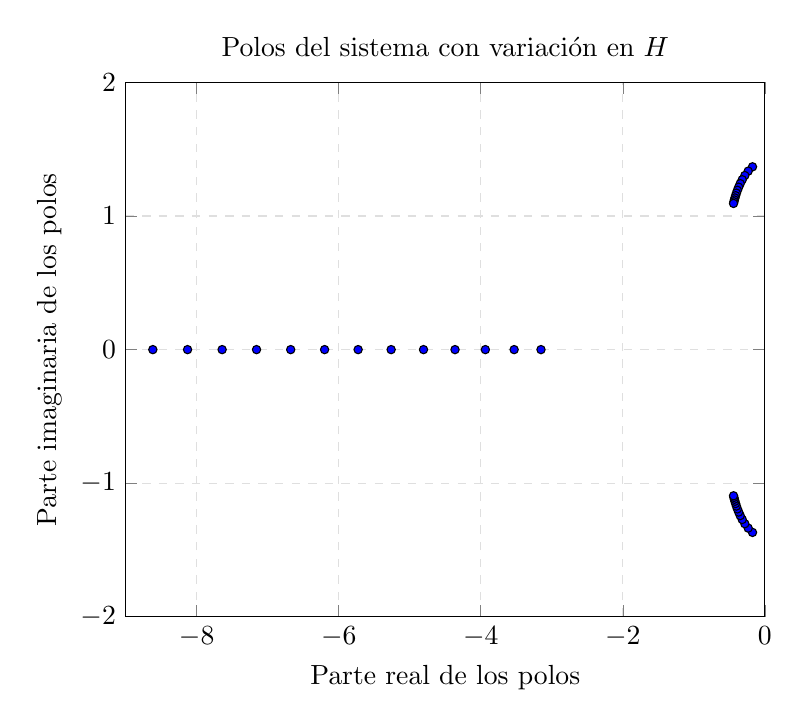
\begin{tikzpicture}
        \begin{axis}[
            width = 0.8\textwidth,
            xmin = -9,
            xmax = 0,
            ymin = -2, ymax = 2,
            grid = both,
            grid style = {gray!25, dashed},
            xlabel = {Parte real de los polos},
            ylabel = {Parte imaginaria de los polos},
            title = {Polos del sistema con variación en $H$}
        ]
            % Polo real
            \addplot[only marks, mark=*, mark options={fill=blue}, mark size=1.5pt]
                coordinates {
                    (-3.1521, 0.0000)
                    (-3.5301, 0.0000)
                    (-3.9356, 0.0000)
                    (-4.3626, 0.0000)
                    (-4.8060, 0.0000)
                    (-5.2617, 0.0000)
                    (-5.7267, 0.0000)
                    (-6.1986, 0.0000)
                    (-6.6758, 0.0000)
                    (-7.1571, 0.0000)
                    (-7.6415, 0.0000)
                    (-8.1283, 0.0000)
                    (-8.6172, 0.0000)
                };

            % Rama compleja superior
            \addplot[only marks, mark=*, mark options={fill=blue}, mark size=1.5pt]
                coordinates {
                    (-0.1739, 1.3687)
                    (-0.2349, 1.3364)
                    (-0.2822, 1.3035)
                    (-0.3187, 1.2718)
                    (-0.3470, 1.2426)
                    (-0.3691, 1.2162)
                    (-0.3866, 1.1925)
                    (-0.4007, 1.1713)
                    (-0.4121, 1.1524)
                    (-0.4215, 1.1355)
                    (-0.4293, 1.1204)
                    (-0.4358, 1.1067)
                    (-0.4414, 1.0944)
                };

            % Rama compleja inferior (conjugada)
            \addplot[only marks, mark=*, mark options={fill=blue}, mark size=1.5pt]
                coordinates {
                    (-0.1739, -1.3687)
                    (-0.2349, -1.3364)
                    (-0.2822, -1.3035)
                    (-0.3187, -1.2718)
                    (-0.3470, -1.2426)
                    (-0.3691, -1.2162)
                    (-0.3866, -1.1925)
                    (-0.4007, -1.1713)
                    (-0.4121, -1.1524)
                    (-0.4215, -1.1355)
                    (-0.4293, -1.1204)
                    (-0.4358, -1.1067)
                    (-0.4414, -1.0944)
                };
        \end{axis}
    \end{tikzpicture}
    \caption{Lugar geométrico de las raíces del sistema realimentado al variar $H$ entre 3 y 9.}
    \label{fig:1}
\end{figure}


Se observa de la figura que todos los polos se encuentra en el semiplano izquierdo, por lo que el sistema es estable para todo valor de $H$. El código \ref{code1} se muestra el código utilizado.

\begin{lstlisting}[caption = {Código MATLAB para generar el lugar de raíces del sistema $G$}, label = {code1}]
clear all

%{
Primer ejercicio
%}
Gs = tf([1, 1, 1], [1, 0.5, 0, 3]); %sistema de la guía 04
Hs = tf([6], [1]);
feed = feedback(Gs, Hs);
polos = pole(feed);

%%
%{
Segundo ejercicio
%}

fig = figure;
hold on;
grid on;
theme(fig, 'light')
matriz_polos = [];
for c = 3:0.5:9
    i = 1;
    Hs = tf([c], [1]);
    sis = feedback(Gs, Hs);
    polos = pole(sis);
    x = real(polos) ; y = imag(polos);
    disp(x)
    plot(x, y, 'b.', MarkerSize=12)
    axis([-10, 1, -3, 3])
    title(['Polos del sistema con H =', num2str(c)])
    xlabel('Parte real de los polos')
    ylabel('Parte imaginaria de los polos')
    drawnow
    pause(0.1)
    i = i + 1;
end

\end{lstlisting}




Aunque la compilación de ese código genera una animación, son demasiadas líneas para calcular cada polo, además de que generamos un bucle el cual es costoso computacionalmente. La opción más rápida es utilizar \texttt{rlocus(Gs)}.


\begin{figure}[ht!]
    \centering
    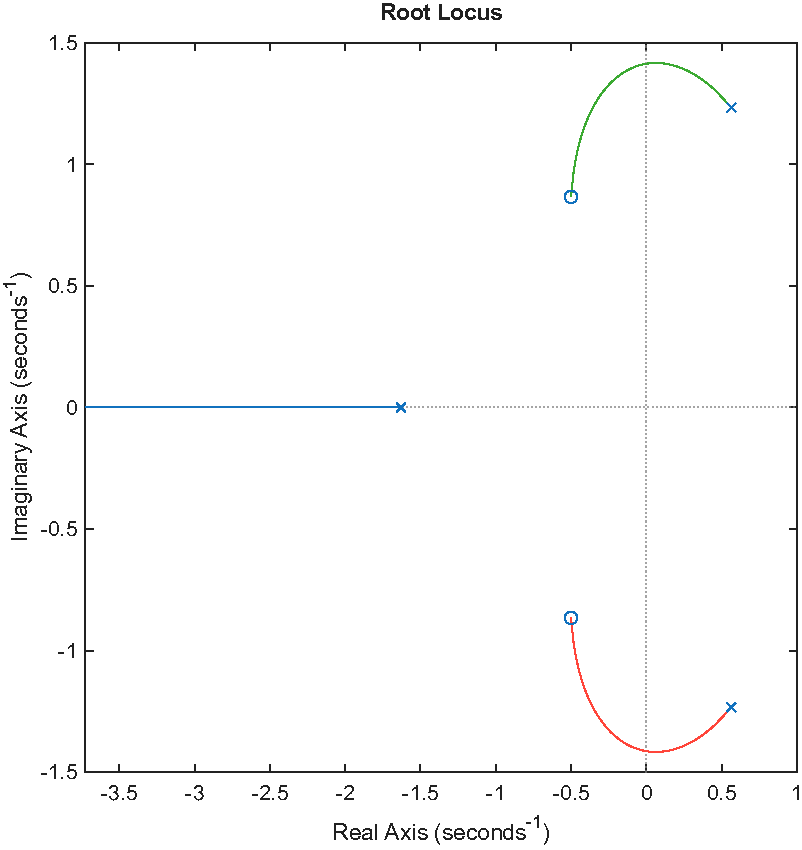
\includegraphics[width=0.8\textwidth]{imagenes/lugar_de_raices.pdf}
    \caption{Lugar de raíces continuo, usando \texttt{rlocus(Gs)}}
    \label{fig:2}
\end{figure}




Para calcular la función de transferencia en lazo cerrado se utiliza la siguiente expresión:


\begin{equation}
    \frac{Y(s)}{R(s)} = \frac{G(s)}{ 1 + G(s)H(s)}
\end{equation}


\noindent Pero también es muy común utilizar la siguiente expresión:


\begin{equation}
    \label{eq:3}
    \frac{Y(s)}{R(s)} = \frac{G(s)H(s)}{ 1 + G(s)H(s)}
\end{equation}


\noindent Si adaptamos el código para este nuevo sistema, el lugar de raíces es:


\begin{figure}[ht!]
    \centering
    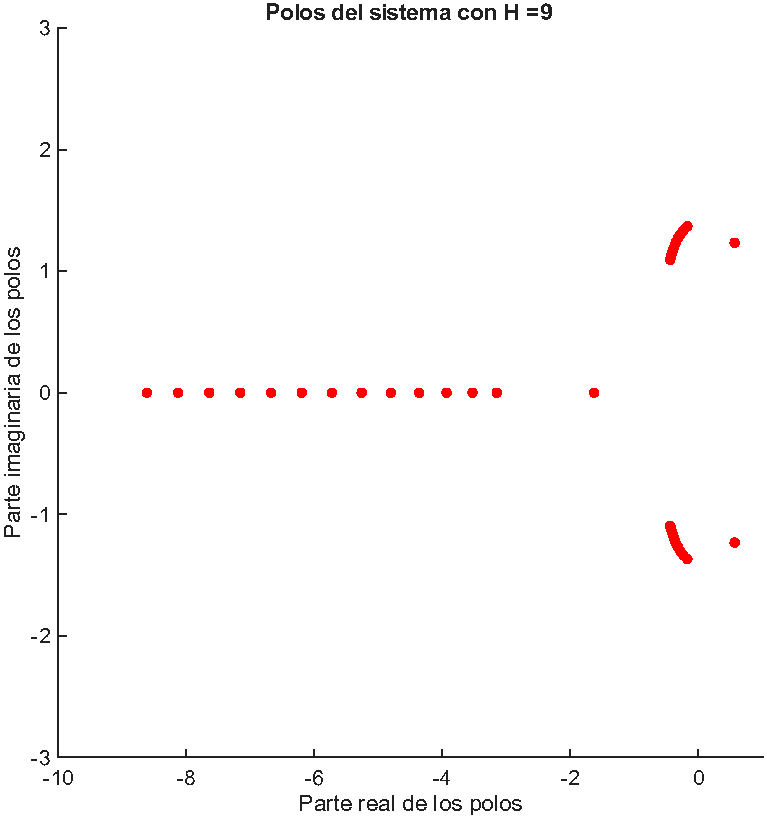
\includegraphics[width=0.8\textwidth]{imagenes/lugar_de_raices2.pdf}
    \caption{Lugar de raíces según la expresión \eqref{eq:3}.}
    \label{fig:}
\end{figure}


No cambia nada con respecto a la figura anterior ya que el denominador no cambió.



Los códigos usados en MATLAB se encuentran debajo:


\begin{lstlisting}[caption = {Código MATLAB para graficar el lugar de raíces}, label = {cod:1}]
clear all

%{
Primer ejercicio
%}
Gs = tf([1, 1, 1], [1, 0.5, 0, 3]); %sistema de la guía 04
Hs = tf([6], [1]);
feed = feedback(Gs, Hs);
polos = pole(feed);

%%
%{
Segundo ejercicio
%}

% fig = figure;
% hold on;
% grid on;
% theme(fig, 'light')
% matriz_polos = [];
% for c = 3:0.5:9
%     i = 1;
%     Hs = tf([c], [1]);
%     sis = feedback(Gs, Hs);
%     polos = pole(sis);
%     x = real(polos) ; y = imag(polos);
%     % disp(x)
%     plot(x, y, 'b.', MarkerSize=12)
%     axis([-10, 1, -3, 3])
%     title(['Polos del sistema con H =', num2str(c)])
%     xlabel('Parte real de los polos')
%     ylabel('Parte imaginaria de los polos')
%     drawnow
%     pause(0.1)
%     i = i + 1;
% end

%{
El código ayuda a ubicar el lugar de raíces.
Me genera una 'animación' a medida que el 
el compensador aumenta de valor. Es estable
para todos los valores; todos se encuentran
en el semiplano izquierdo (estabilidad del
sistema).

Aunque el resultado es lindo, calcular 
de esta forma las raíces del sistema
es laborioso. Por lo tanto, la mejor opción
es usar la función 'rlocus(Gs)' y me grafica
todo el lugar de raíces de dicho sistema.
Aunque la función de rlocus es fácil, no 
presenta la ventaja de cambiar el compensador
%}

% Nuevo Gs
fig2 = figure;
theme(fig2, 'light')
Gs1 = tf([1, 1], [1, 0.5, 0, 3]); 
rlocus(Gs)




%%

%{
Implemento el nuevo sistema G*H/(1+G*H)
Es prácticamente lo mismo que el sistema
anterior.
%}
fig3 = figure;
theme(fig3, 'light')
hold on;
for c = 3:0.5:9
    Hs = tf([c], [1]);
    new_sis = Gs*Hs/(1+Gs*Hs);
    polos = pole(new_sis);
    x = real(polos) ; y = imag(polos);
    plot(x, y, 'r.', MarkerSize=12)
    axis([-10, 1, -3, 3])
    title(['Polos del sistema con H =', num2str(c)])
    xlabel('Parte real de los polos')
    ylabel('Parte imaginaria de los polos')
    drawnow
    pause(0.1)
end
\end{lstlisting}

